\documentclass{beamer}

%%% -------------- CREATE HANDOUTS -----------------------------------
%\documentclass[12pt, handout]{beamer}
%\usepackage{pgfpages}
%\pgfpagesuselayout{4 on 1}[letterpaper, landscape, border shrink=5mm]
%%% ------------------------------------------------------------------


\mode<presentation>
  \usepackage{ru}
  %\usetheme{Warsaw}
  %\usecolortheme{seahorse}
  %\usefonttheme{default}
  \setbeamertemplate{caption}[numbered]
  %\setbeamertemplate{navigation symbols}{}
  \setbeamertemplate{bibliography item}[text]
\newcommand*\oldmacro{}%
	\let\oldmacro\insertshorttitle%
%\renewcommand*\insertshorttitle{%
%   \oldmacro\hfill%
%   \insertframenumber\,/\,\inserttotalframenumber}
\setbeamertemplate{section page}{
    \begin{centering}
    \vspace{1cm}
    \begin{beamercolorbox}[rounded=true,shadow=false,sep=4pt,center]{part title}
    \usebeamerfont{section title}\LARGE{\insertsection}\par
    \end{beamercolorbox}
    \end{centering}}
\usepackage{ragged2e}
\usepackage[english]{babel}
\usepackage[utf8]{inputenc}
\usepackage{appendixnumberbeamer}
\usepackage{natbib}
\usepackage{textpos}
\usepackage{lipsum}
\usepackage{tikz}
\usepackage[percent]{overpic}
\usepackage{textcomp}
\usepackage{booktabs}
\usepackage{mathabx}
\usepackage{pifont}
\usepackage{bbding}
\usepackage{fontenc}
%\let\Sun\undefined   %to undefine something
%\usepackage{marvosym}
%\usepackage{scalerel}
%% \usepackage[
%%   style=numeric,
%%   citestyle=authoryeartitle
%% ]{biblatex}
\setbeamerfont{caption}{size=\tiny}

%\setbeameroption{show notes}
%\setbeamertemplate{note page}[plain]
\newcommand{\tss}{\textsuperscript}
\newcommand{\tsbs}{\textsubscript}
%Change Bullets in latex list
\setbeamertemplate{itemize item}{\scriptsize\raise1.25pt\hbox{\donotcoloroutermaths\ding{118}}}
\setbeamertemplate{itemize subitem}{\scriptsize\raise1.25pt\hbox{\ding{226}}}
\setbeamertemplate{itemize subsubitem}{\tiny\raise1.25pt\hbox{\ding{169}}}
\setbeamertemplate{enumerate item}{\insertenumlabel.}


%%To select specific font
%{\fontsize{2.5}{4}\selectfont tobesize}

%\setbeamertemplate{background}{\tikz[overlay, remember picture]\node[xshift=-2.3cm, yshift=1.50cm, opacity=0.4]at (current page.south east){
\includegraphics[width=4cm]{images}};}

\title[Cycle 1]{The First Cycle Status}
\author{Paul Mendoza}
\date{October 12, 2016}

\begin{document}
\setbeamertemplate{caption}{\raggedright\insertcaption\par}
\begin{frame}
	%% background
  \tikz[overlay, remember picture]\node[xshift=-3.5cm, yshift=3cm, opacity=0.1]at (current page.south east){
\includegraphics[width=8cm]{tamu_system_proposed_seal_042915}};
	%% Left-hand logo
  %% \begin{tikzpicture}[remember picture, overlay]
  %% \node [xshift = 3 cm, yshift=1.2cm] at (current page.south west){
\includegraphics[width=5cm]{tees_logo_primary_maroon}};
  %% \end{tikzpicture}
    %% Right-hand logo
  \begin{tikzpicture}[remember picture, overlay]
  \node [xshift = -3cm, yshift=1.2cm] at (current page.south east){
\includegraphics[width=5cm]{TEES_NSSPI_logo_HMaroon}};
  \end{tikzpicture}
  %% Upper logo right
    %% \begin{tikzpicture}[remember picture,overlay]
    %% \node[anchor=north east,yshift=2pt] at (current page.north east) {
\includegraphics[height=0.8cm]{NUENlogo}};
    %% \end{tikzpicture}
  %% Upper logo left
    %% \begin{tikzpicture}[remember picture,overlay]
    %% \node[anchor=north west,yshift=2pt] at (current page.north west) {
\includegraphics[height=0.8cm]{NUENlogo}};
    %% \end{tikzpicture}
    \titlepage
    \vspace{-1.8cm}
    \begin{center}
      Presented at Research Meeting
    \end{center}
\end{frame}

%Add Biola Seal
%% \setbeamertemplate{background}{\tikz[overlay, remember picture]\node[xshift=-2.5cm, yshift=2.5cm, opacity=0.05]at (current page.south east){
\includegraphics[width=6cm]{imageedit_2_7317234434}};}

%Add NSSPI to upper right
%% \addtobeamertemplate{frametitle}{}{%
%%   \begin{tikzpicture}[remember picture,overlay]
%%     \node[anchor=north east,yshift=2pt] at (current page.north east) {
\includegraphics[height=0.8cm]{TEES_NSSPI_Acronym_logo_WHT}};
%%     \end{tikzpicture}}



%% \begin{frame}{Outline}
%% \tableofcontents
%% \end{frame}

\section{Status of Experiment}
\begin{frame}{Things Counting}
  %\vspace{-1cm}
  \begin{figure}[H] % Example of including images
    \begin{center}
      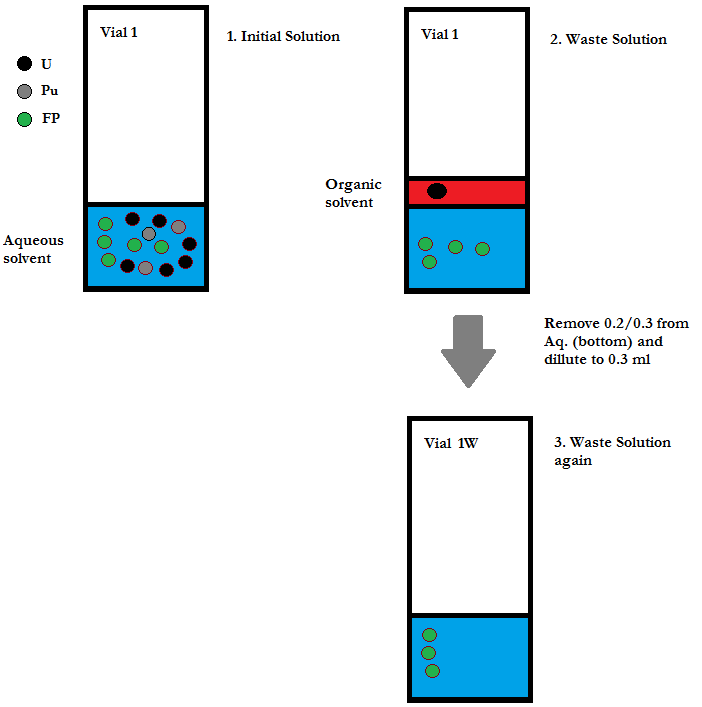
\includegraphics[width=0.6\linewidth]
                      {Extraction_Cycle_1_First_3_Counts}
    \end{center}
    \caption{First Three Counts}
  \end{figure}  
\end{frame}

\begin{frame}{Things Counting}
  \begin{figure}[H] % Example of including images
    \begin{center}
      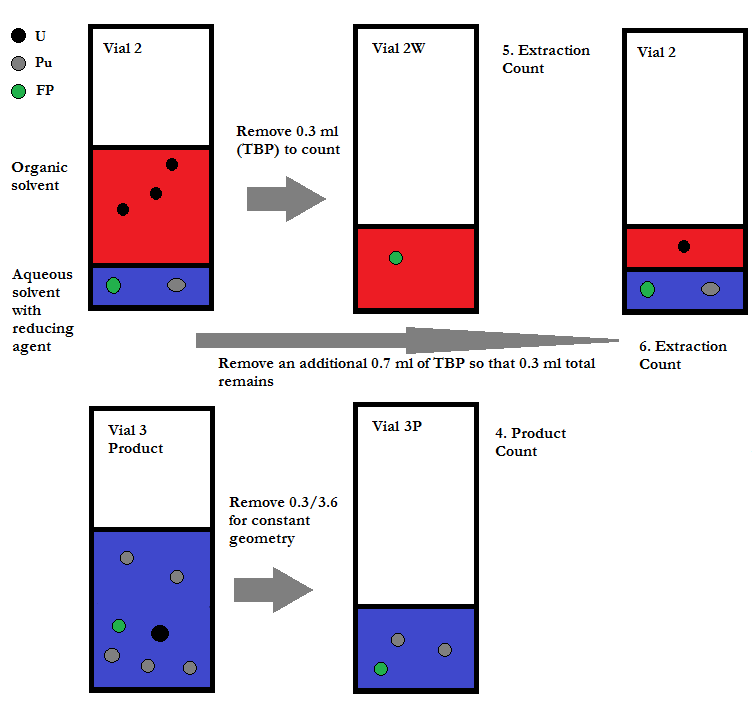
\includegraphics[width=0.6\linewidth]
                      {Back_Extraction_Cycle_1_Last_3_Counts}
    \end{center}
    \caption{Second Three Counts}
  \end{figure}
\end{frame}

\section{Preliminary Results}
\begin{frame}{Preliminary Results}
  \vspace{-0.6cm}
  \begin{block}{Activity Reduction}
    \begin{center}
      \vskip -0.2cm
  {\fontsize{7}{11.2}\selectfont
  \begin{tabular}{l  c  c c c c}\toprule
   Isotope & Reduction & Error \\ \midrule 
   Rb(37) & 39.0 & 5.9  \\
   Sr(38) & 283  & 43   \\
   Mo(42) & 5.7  & 0.8  \\
   Ru(44) & 59.2 & 6.4  \\
   Pd(46) & 65   & 14   \\
   Cd(48) & 74   & 17   \\
   Cs(55) & 177  & 28   \\
   Ce(58) & 43   & 16   \\
   Nd(60) & 19.2 & 2.1  \\
   Pm(61) & 12.8 & 1.9  \\
   Sm(62) & 11.5 & 1.5  \\
   Eu(63) & 10.0 & 1.4  \\
   U(92) & 7.4   & 1.2  \\ \bottomrule
  \end{tabular}
  }
  \end{center}
  \end{block}
\end{frame}

\section{Next Week}
\begin{frame}{Next Week}
  \begin{itemize}
  \item{Analysis of first cycle, with alpha}
  \item{Second Cycle complete (experiment)}
  \end{itemize}
\end{frame}

\end{document}
